\documentclass[twocolumn,aps]{revtex4}

\usepackage{graphicx}

\newcommand{\cernvm}{CernVM}
\newcommand{\cernvmgraphics}{\cernvm{}-Graphics}
\newcommand{\cernvmwrapper}{\cernvm{}-Wrapper}
\newcommand{\boinc}{BOINC}
\newcommand{\opengl}{OpenGL}
\newcommand{\virtualbox}{VirtualBox}
\newcommand{\curl}{cURL}
\newcommand{\json}{JSON}
\newcommand{\vmport}{12345}
\newcommand{\einsteinathome}{Einstein@Home}
\newcommand{\jquery}{jQuery}

\begin{document}

  \title
  {
    \cernvmgraphics{} - An extensible, configurable graphics application to 
    be used with the \boinc{}-\cernvm{} framework 
  }

  \date{ September 1 2011 }
  \author{ Ben Page }
  \noaffiliation

  \begin{abstract}
    \cernvmgraphics{} is a cross platform application designed to create a 
    visual display for \cernvm{}-based physics applications distributed by 
    the \boinc{} infrastructure. It is based upon web technologies such as 
    HTTP and \json{} to simplify laying out displays and is designed to ease
    the addition of extra functionality.
    This paper presents an overview of the development of \cernvmgraphics{}.
    It covers the original motivation for the graphics application, the
    constraints laid out by the framework, the design decisions made in 
    the development and an overview of the classes employed.
  \end{abstract}

  \maketitle

  \section{ Overview }
    In recent years projects have been underway to allow physicists to use
    the distributed computing infrastructure \boinc{} 
    \cite{boincIntroduction} to utilise cheaply volunteer computers for 
    purposes of both calculation and outreach. Physics code often lacks 
    portability and as a large fraction of volunteers will be using a 
    different platform than the developers (Windows rather than Linux) the 
    community has begun to use virtual machines to distribute and run the 
    code. This, however, presents a usability problem to any non-physicist.
    Most users expect computers to provide GUIs, but any physics code
    running on a virtual machine is written for the terminal, which is not 
    commonly regarded as visually appealing. \cernvmgraphics{} is the result
    of a will to solve this difficulty within the system presented by both 
    \boinc{} and \cernvm{} \cite{cernvmIntroduction}. A screenshot of the 
    package is in figure \ref{screenshot}.

    \begin{figure}[hbt]
      \label{screenshot}
      \centering
        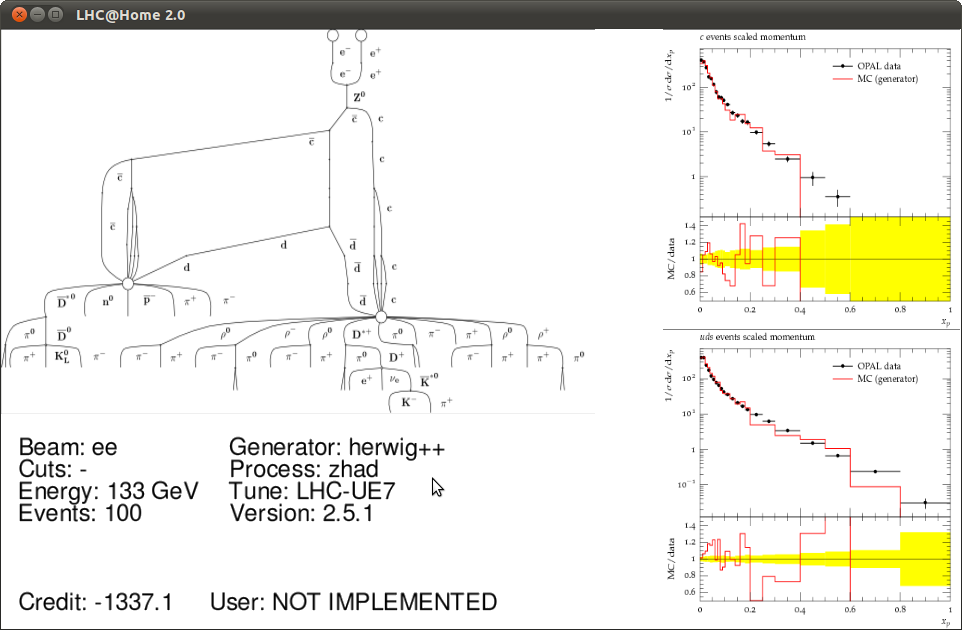
\includegraphics[width=0.45\textwidth]{graphics/screenshot.png}
      \caption
      {
        A screenshot of a simple setup within \cernvmgraphics{} with a
        picture, a ``gridshow'', some metadata and \boinc{} information 
        objects.
      }
    \end{figure}


    The constraints that dictated the direction of the project were laid out
    by this framework.  \boinc{} was designed to be cross-platform and so 
    \cernvmgraphics{} had to follow its lead. However, \boinc{} provides a 
    collection of tools to create cross platform graphics applications,
    which include \opengl{} and \curl{}. From this grounding we have built
    \cernvmgraphics{} to be an easily configurable, with \json{}, graphics 
    application that takes its configuration and resources from within a 
    \cernvm{} virtual machine by means of HTTP transfer. 
    
    \cernvmgraphics{} now joins the \cernvm{}/\boinc{} structure in a way
    described in figure \ref{structure}.

    \begin{figure}[hbt]
      \label{structure}
      \centering

      \setlength{\unitlength}{0.45\textwidth}
      \begin{picture}(1, 1)
        %Top Level (BOINC)
        \put(0.3, 0.8){ \framebox(0.4, 0.2){\boinc{}} }

        \put(0.52, 0.71){ \makebox{ \boinc{} bindings } }
        \put(0.5, 0.65){ \vector(0,  1){0.15} }
        \put(0.5, 0.8){ \vector(0, -1){0.15} }

        %Middle Level (Cernvm-Wrapper)
        \put(0, 0.45){ \framebox(1, 0.2){\cernvmwrapper{}} }

        \put(0.07, 0.36){ \makebox{ VBoxManage } }
        \put(0.05, 0.45){ \vector(0, -1){0.15} }

        \put(0.67, 0.36){ \makebox{ Shared Memory } }
        \put(0.65, 0.45){ \vector(0, -1){0.15} }
        \put(0.65, 0.3){ \vector(0,  1){0.15} }

        %Bottom Level (CernVM and CernVM-Graphics)
        \put(0, 0)
        {
          %virtualbox
          \put(0, 0.225){\makebox(0.4, 0.075){\virtualbox{}}}
          \multiput(0.4,0)(0, 0.04){8}{\line(0,1){0.02} }
          \put(0,0){\line(0,1){0.3}}
          \put(0,0){\line(1,0){0.4}}
          \put(0,0.3){\line(1,0){0.4}}

          %cernvm box
          \put(0.04,0.025){ \framebox(0.3, 0.2){\cernvm{}} }

          \put(0.42, 0.17){ \makebox{HTTP} }
          \put(0.34, 0.15){ \vector( 1, 0) {0.26} }
          \put(0.60, 0.15){ \vector(-1, 0) {0.26} }

          %cernvmGraphics
          \put(0.6,0){ \framebox(0.4, 0.3){\cernvmgraphics{}} }
        }

      \end{picture}

      \caption
      {
        A diagram of the current structure of the LHC@Home project and
        \cernvmgraphics{} place in it. Arrows indicate communication
        between layers (with directionality). \virtualbox{} 
        \cite{virtualbox} itself contains the \cernvm{} image but allows 
        direct communication with the VM via HTTP.
      }
    \end{figure}



  \section{ Design Decisions }
    We began with a will to replicate a simple slideshow screensaver, moving
    through a selection of physics images. Though the power that \opengl{} 
    provides is great, the code required to display a simple 2D image is 
    quite long - providing features that are commonly unnecessary. 
    Therefore we created our first abstraction - the sprite class. In short 
    it provides the developer the ability to import a PNG image and display 
    it on the screen using either ``window-fraction'' or ``pixel-based'' 
    coordinates. In providing such a wrapping around \opengl{} textures, 
    however, it has been neglected to provide a copy constructor for the 
    class - principally because the developer believes that such large 
    objects should not be copied in this context, only passed around by 
    reference. To this end utility functions are provided to manage storage 
    of sprites. Sprites are stored and referenced in ``groups'', which are
    simply C++ maps of strings to ``Sprite*''. Groups are provided as an
    abstraction as often, in real usage cases, groups of sprites are
    required for things like slideshows.

    As the project progressed it was unclear what exact ``objects'' would be
    placed upon the \cernvmgraphics{} window and so the decision was make
    to provide exactly this abstraction to the developer. \cernvmgraphics{}
    provides an ``Object'' class from which all useful objects are
    descended. These children are meant to provide both a constructor, which
    accepts a \json{} node that describes the object, and a render function,
    which acts appropriately on the provided description. Instances of these
    children are stored in a vector which calls each render function once 
    every frame.

    For this display to replace completely a \cernvm{} terminal window (and 
    especially in the case of the user) we realised that we needed a way to 
    show an error output. What's more, it would be quite useful for a 
    user to be able to press a key and be able to see different information
    - for example, providing an explanation of the physics pictures or
    separating \boinc{} user information from the physics; this provoked the
    idea of ``views''. Previously only one collection of objects  could be 
    shown at one time, but with views we chose to allow the user to press
    a number key to swap the displayed collection (this constraint on keys a
    testimony to the developer's lack of imagination). Internally, objects
    are stored within views with there being an active view pointer, which
    is changed upon a key press.

    In order to keep this extensible and easily configurable an external
    ``config'' file is loaded, called index.json (as a reference to HTML),
    the specification of which is presented with the package.  \json{} was 
    chosen as the file format because of the ease of reading and writing 
    \json{} (compared to XML) and also looking forward to web based 
    implementations of \cernvmgraphics{} as \json{} is widely supported due 
    to its close links to javascript. During development it was noted that
    the display designer may not be the same person providing the physics
    resources, so these can be externalised to resource \json{} files to
    avoid confusing the resource provider with the display semantics.
    To facilitate incorporation of these resources in the program there are 
    helper functions to ease access to them under their global names.

    The next key decision was to specify the method of communication
    between \cernvm{} and \cernvmgraphics{}. A VM naturally believes itself
    to be a real computer, and so any good method of communicating would 
    mirror normal communication with a computer. To this end we opted to
    communicate via HTTP, having \cernvm{} serve the configuration and all
    other resources through port \vmport{}. This port was chosen at random
    to avoid using 8080 as some users may have their own web server on this
    port. \cernvmgraphics{} now accesses localhost:\vmport{} to find its
    resources, but it would not be difficult to point to any web address.

    The technology used to get these files from \cernvm{} was dictated by
    the constraints of staying within \boinc{}'s framework, and so we chose
    \curl{} (provided by \boinc{}). The complications of \curl{}'s usage
    were enough that the developer chose to abstract it away into a
    ``FileDownloader'' class. This provides an easy way to perform either
    synchronous or asynchronous file downloads, with the latter being
    processed in the main graphics loop. \cernvmgraphics{} is capable of 
    checking for new display information from \cernvm{} at a given interval,
    however the method of detecting if the information is new is not robust.
    The standard method of deciding this is to check the remote file's
    modification timestamp, but the notion of `time' within a VM is 
    difficult as any pausing/resuming will cause a de-sync with host time. 
    The solution to this problem is to redownload the \json{} files, and
    compare them against the old ones. These files are only small and so do
    not greatly limit the rate of refreshing.

    The configuration of all these abstractions can be found in the
    documentation provided with the package.
    
    Later in development it was noted that in order for \cernvmgraphics{} to
    be usable as a \boinc{} screensaver, it would be necessary for the
    display to be resolution independent - that it should scale. This was
    easily achievable with \opengl{} as it naturally supports coordinates as
    fractions of the window, and so \cernvmgraphics{} supports both
    ``normalised'' and ``non-normalised'' coordinates. To make sure that any
    given display looks the same on any given monitor we had to set the
    aspect ratio which the ``normalised'' coordinates were based upon.
    There is no one ubiquitous monitor aspect ratio so the decision was made
    to choose one that fits in the middle and we settled on 16:10.

  \section{ The Future }
    The future of \cernvmgraphics{} is very broad, as the technologies it is
    build on are very powerful, but it has also been built to be 
    extensible/easily configurable. In this vein it is quite probable that
    the developers eye was not keen enough to make everything configurable.
    However for the broader picture there are some large, exciting changes
    that could be useful to provide. For example, \opengl{} is a 3D library
    which has been used only in a 2D way, but it would also be possible to
    add 3D functionality (similar to \einsteinathome{} \cite{einsteinathome}
    ). One potential criticism to address is that \cernvmgraphics has been
    written with web technologies in mind, but if one were to point your
    browser to localhost:\vmport{} one would get nothing back. One
    proposition would be to port \cernvmgraphics{} to javascript in order to
    levee the natural HTTP capabilities as well as ease of \json{} parsing.
    Technologies such as \jquery{} \cite{jquery} could help provide 
    cross-browser compatibility; what's more \jquery{} plugins, e.g. cycle
    \cite{jquery-cycle}, provide ready made user interface technology.

  \section{ Conclusions }
    \cernvmgraphics is an easily configurable, extensible solution to the
    problem presented by \cernvm{}'s terminal's usability. It is written in
    such a way to allow easy addition of features and the project has many 
    paths it can follow in the future.

  \begin{thebibliography}{9}

    \bibitem{boincIntroduction}
      \boinc{} - http://boinc.berkeley.edu

    \bibitem{cernvmIntroduction}
      \cernvm{} - http://cernvm.cern.ch

    \bibitem{virtualbox}
      \virtualbox{} - http://www.virtualbox.org

    \bibitem{einsteinathome}
      \einsteinathome{} - http://einstein.phys.uwm.edu

    \bibitem{jquery}
      \jquery{} - http://www.jquery.com

    \bibitem{jquery-cycle}
      \jquery{} Cycle - http://jquery.malsup.com/cycle

  \end{thebibliography}

\end{document}
